\subsubsubsection{Scheduling}
The scheduling package contains all the logic needed to have worker threads
which consume work items, which correspond to the actions that occur in our
simulations.

The scheduling system instantiates two executors, one for the travellers and
one for traffic lights: this is done to minimize time drifts among different
traffic lights (which can toggle their state smoother, without having to
compete with travellers to be dequeued and executed).
However, these two executors are the same package, just instantiated twice with
a different number of worker threads.

We will present our scheduling component by first describing how our system
starts, then how it executes work items and how it stops.
Finally, we will have a quick look at the \texttt{Callback} hierarachy.

\paragraph{Start}

Scheduling is started asynchronously by providing a list of work items
(or \textit{agenda}), which correspond to either travellers' or traffic
lights' actions.
Scheduling will just process this list, by registering events at the time
reported in the agenda.

\paragraph{Execution}

% TODO: Fix
In Figure \ref{fig:schedule-workflow} we show how a request to schedule an
entity is handled:

\begin{enumerate}
  \item First, the \texttt{Scheduler} delegates the execution of an action to an
    \texttt{Executor}: the latter is an interface which is implemented by
    \texttt{SimpleExecutor} in our system;
  \item \texttt{SimpleExecutor} registrates a timer to defer the action;
  \item When the timer expires, it asks to its \texttt{Executor} reference to
    execute an action (the one which originally had to be scheduled);
  \item If it is not stopped, \texttt{SimpleExecutor} add this action to the
    \texttt{WorkQueue}
  \item and notifies the \texttt{CommandBroker} that there is new work;
  \item This causes the \texttt{CommandBroker} to open a guard and makes the
    \texttt{WorkerThread}(s) wake up;
  \item Each one of the \texttt{WorkerThread}s asks for item, consuming them
    until there is some.
\end{enumerate}

\begin{figure}[H]
\centering
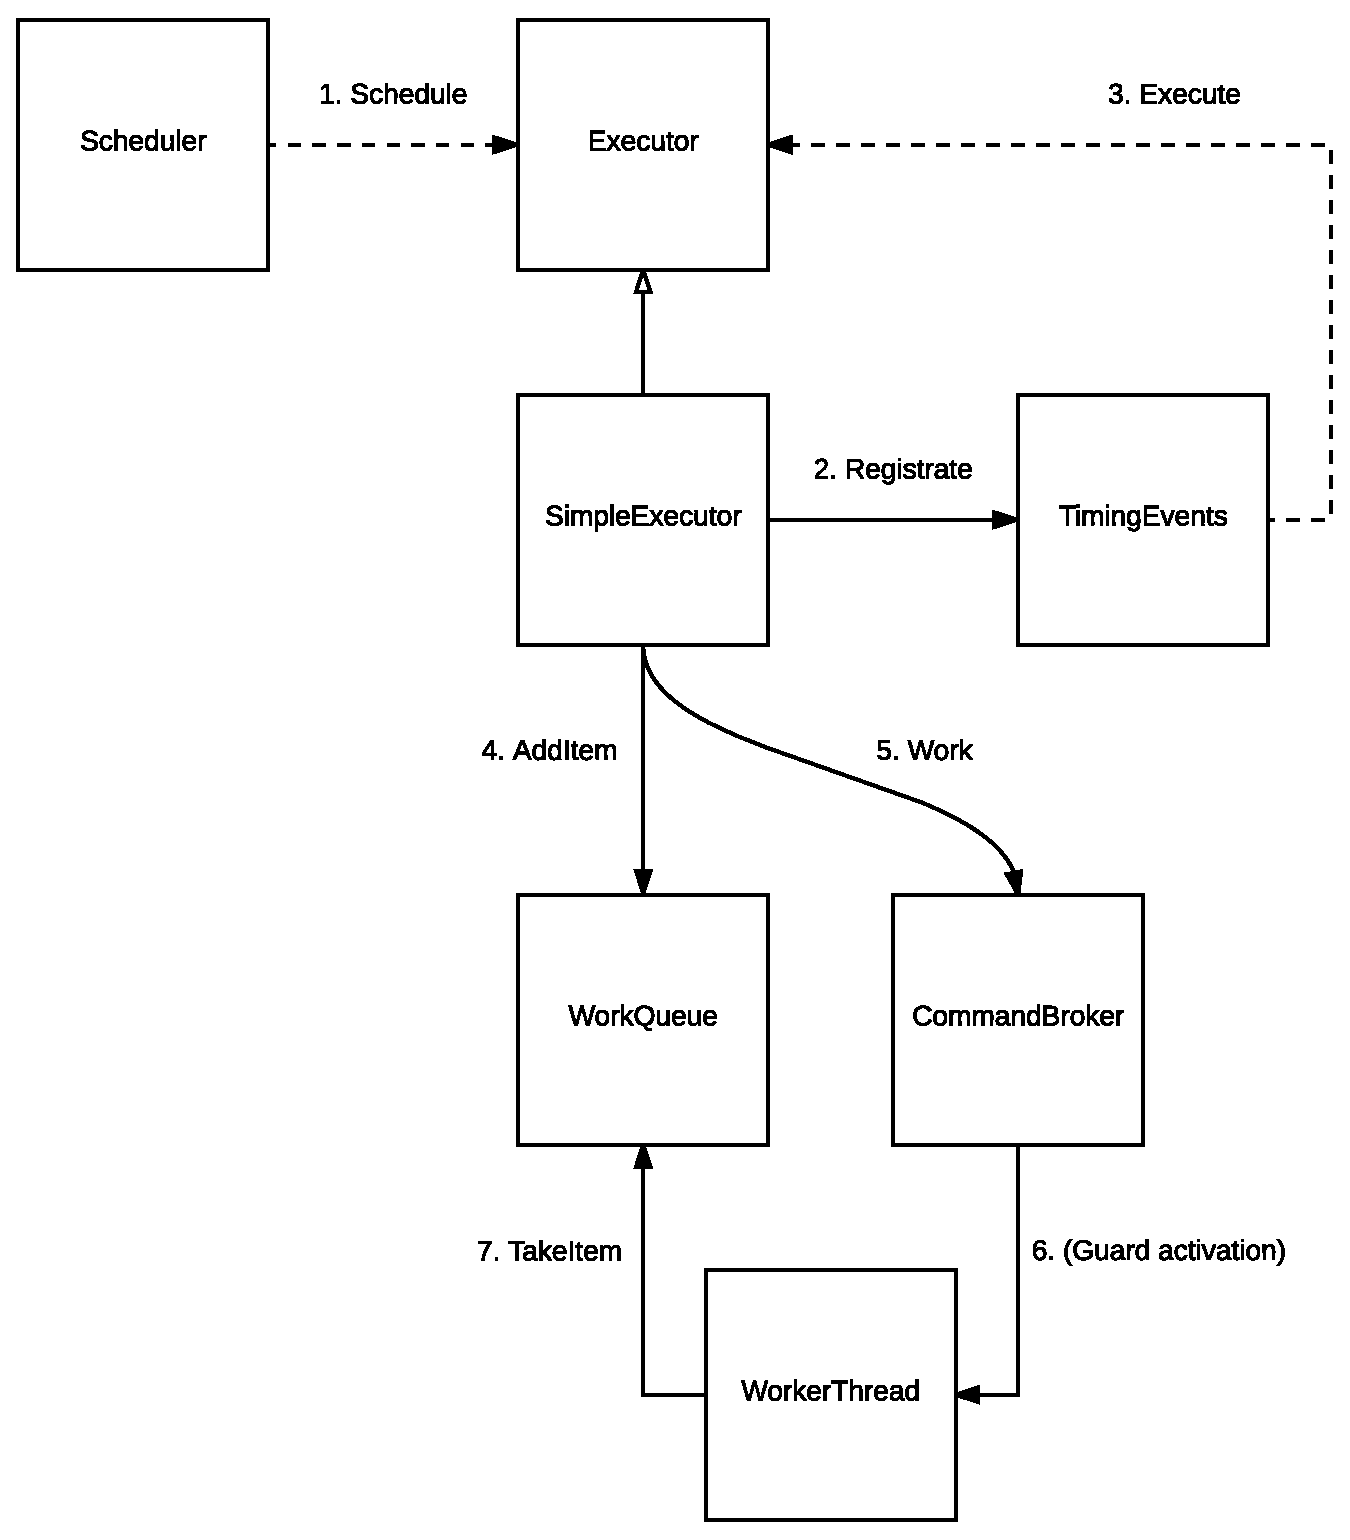
\includegraphics[scale=0.4,keepaspectratio]{images/solution/app/backend/scheduler.eps}
\caption{Schedule workflow}
\label{fig:schedule-workflow}
\end{figure}

\paragraph{Termination}

% TODO: Fix
BLA BLA BLA TERMINATION...

\paragraph{Callbacks}

% TODO: Fix
BLA BLA BLA CALLBACKS...
